\documentclass[a0,portrait]{a0poster}

\usepackage[margin=1.5cm]{geometry}
\usepackage[utf8]{inputenc}
\usepackage[T1]{fontenc}
\usepackage{lmodern}
\usepackage{amsmath,amssymb}
\usepackage{booktabs}
\usepackage{array}
\usepackage{graphicx}
\usepackage{xcolor}
\usepackage{tikz}
\usepackage{multicol}
\usepackage{enumitem}
\usetikzlibrary{arrows.meta,positioning,calc}

\graphicspath{{figures/}{template_assets/}}

% Paleta do MODELO DE SLIDE (InovAI Lab)
\definecolor{PmPurple}{HTML}{3C23A3}
\definecolor{PmPurpleSoft}{HTML}{858DFD}
\definecolor{PmLilac}{HTML}{A69FFD}
\definecolor{PmBlue}{HTML}{4285F4}
\definecolor{PmCyan}{HTML}{0097A7}
\definecolor{PmOrange}{HTML}{FFAB40}
\definecolor{PmCanvas}{HTML}{F7F6FC}
\definecolor{PmInk}{HTML}{212121}
\definecolor{PmMuted}{HTML}{78909C}
\definecolor{PmLine}{HTML}{E4E0F5}
\definecolor{PmWhite}{RGB}{255,255,255}
\colorlet{PmCarapace}{PmPurple}
\colorlet{PmVenom}{PmPurpleSoft}
\colorlet{PmVenomDeep}{PmOrange}
\colorlet{PmMembrane}{PmBlue}
\colorlet{PmGreen}{PmCyan}

\pagecolor{PmCanvas}
\color{PmInk}
\setlength{\columnsep}{0.75cm}
\setlength{\parindent}{0pt}
\setlist[itemize]{leftmargin=1.0em, itemsep=0.12em, topsep=0.1em}
\setlist[enumerate]{leftmargin=1.1em, itemsep=0.12em, topsep=0.1em}

\newcommand{\sectionbox}[2]{%
  \vspace{0.10cm}%
  \noindent
  \begin{tikzpicture}
    \node[
      draw=PmLine, fill=PmWhite, rounded corners=3pt,
      inner sep=9pt, text width=\dimexpr\linewidth-24pt\relax,
      align=left
    ] {
      {\color{PmPurple}\Large\bfseries #1}\\[0.18em]
      {\color{PmPurple}\rule{2.6cm}{2.4pt}\color{PmPurpleSoft}\rule{0.7cm}{2.4pt}\color{PmBlue}\rule{0.45cm}{2.4pt}}\\[0.28em]
      #2
    };
  \end{tikzpicture}%
}

\newcommand{\metriccard}[3]{%
  \begin{tikzpicture}
    \node[
      draw=PmLine, fill=PmWhite, rounded corners=3pt,
      align=center, minimum width=8.8cm, minimum height=3.1cm,
      inner sep=8pt
    ] {
      {\color{PmMuted}\small #1}\\[0.1em]
      {\color{#3}\fontsize{34}{38}\selectfont\bfseries #2}\\[0.05em]
      {\small LOPO AUC}
    };
  \end{tikzpicture}%
}

\begin{document}

% ===================== CABEÇALHO =====================
\noindent
\begin{tikzpicture}
  \node[fill=PmPurple, rounded corners=3pt, inner sep=0pt,
        minimum width=0.995\linewidth, minimum height=7.0cm] (hdr) {};
  \fill[PmPurpleSoft, opacity=0.28] ([xshift=5cm,yshift=-1.2cm]hdr.north west) circle (5.2cm);
  \fill[PmBlue, opacity=0.18] ([xshift=-3cm,yshift=1cm]hdr.south east) circle (5.0cm);
  \fill[PmLilac, opacity=0.22] ([xshift=10cm,yshift=-2cm]hdr.north west) circle (3.6cm);
  \fill[PmPurpleSoft] ([yshift=0.28cm]hdr.south west) rectangle ([yshift=0.48cm]hdr.south east);
  \node[anchor=north west, xshift=0.55cm, yshift=-0.4cm,
        fill=white, rounded corners=2pt, inner sep=4pt] at (hdr.north west) {%
    
\includegraphics[height=1.15cm]{logo_inovai.png}%
  };
  \node[anchor=north east, xshift=-0.55cm, yshift=-0.4cm,
        fill=white, rounded corners=2pt, inner sep=4pt] at (hdr.north east) {%
    
\includegraphics[height=1.05cm]{logo_ufrn.png}%
  };
  \node[anchor=north, text width=0.68\linewidth, align=center] at ([yshift=-1.75cm]hdr.north) {
    {\color{PmLilac}\large\bfseries INOVAI LAB \;$\cdot$\; LANCE \;$\cdot$\; IMD/UFRN}\\[0.28em]
    {\color{PmWhite}\fontsize{30}{34}\selectfont\bfseries PepMem-AI: predição de interação peptídeo--membrana}\\[0.12em]
    {\color{PmWhite}\large para priorização de peptídeos escorpiônicos (\emph{Tityus stigmurus})}\\[0.22em]
    {\color{white!90}\normalsize Projeto CNPq de bioprospecção --- Universidade Federal do Rio Grande do Norte --- 2026}
  };
\end{tikzpicture}

\vspace{0.2cm}

\begin{multicols}{3}

% ---------- COL 1 ----------
\sectionbox{1. Problema e objetivo}{
Peptídeos de peçonha (Stigmurin e análogos) atuam em membranas diversas (Gram+/Gram$-$, fungo, célula mamífera). Ensaios MIC exaustivos são caros.

\vspace{0.2em}
\begin{center}

\begin{tikzpicture}
  \node[draw=PmVenom, fill=PmCarapace, text=PmWhite, rounded corners=3pt,
        align=center, inner sep=10pt, text width=0.92\linewidth] {
    \textbf{Pergunta do PoC}\\[0.15em]
    Chance de \textcolor{PmVenom}{alta atividade} (MIC $\le$ 3,4\,µM)\\
    para um peptídeo $\times$ membrana?
  };
\end{tikzpicture}
\end{center}
\vspace{0.15em}
{\small Prioriza candidatos; \textbf{não} substitui bancada/clínica.}
}

\sectionbox{2. Dados e rótulo}{
\begin{itemize}
  \item \textbf{90} pares MIC · \textbf{10} peptídeos · \textbf{18} alvos
  \item \textbf{78} bancada + \textbf{12} literatura (bancada sobrescreve)
  \item Positivos (MIC $\le$ 3,4\,µM): $\approx$\textbf{44\%}
\end{itemize}
\vspace{0.15em}
\begin{center}
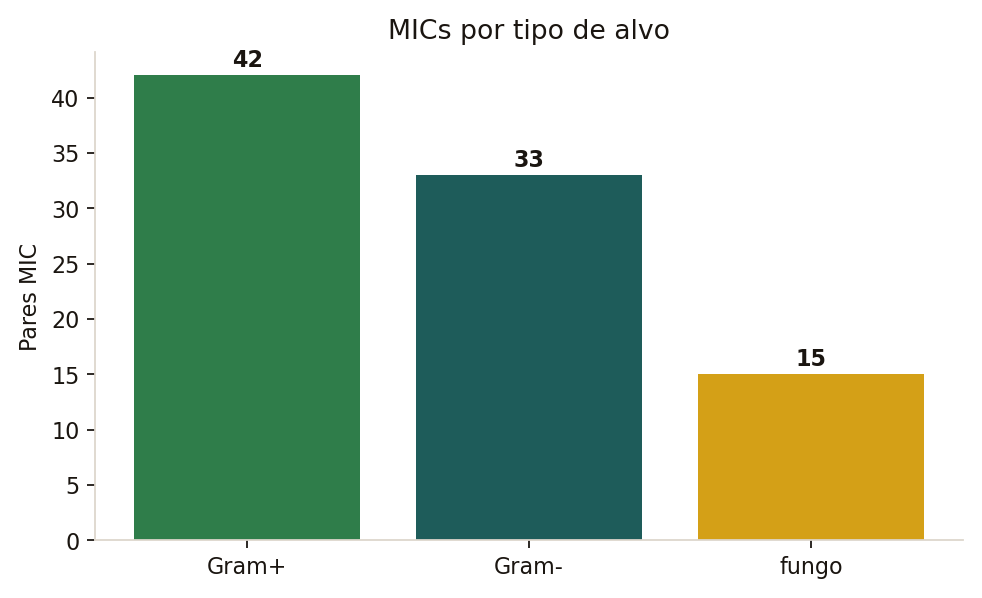
\includegraphics[width=0.95\linewidth]{mic_por_tipo.png}\\[0.12em]
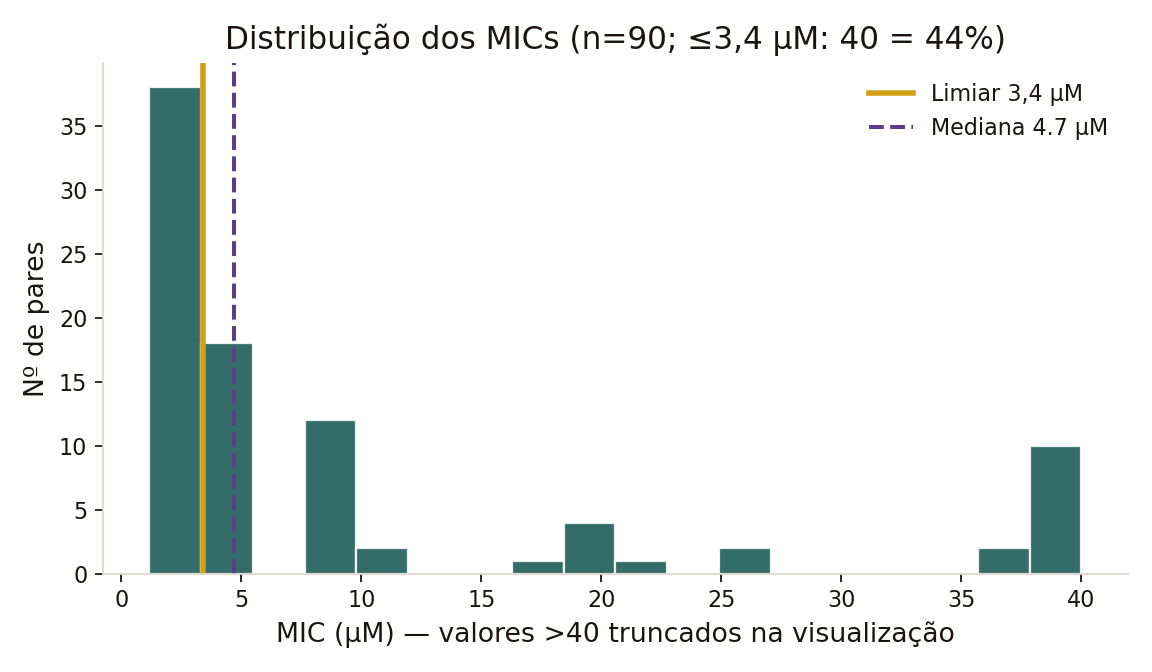
\includegraphics[width=0.95\linewidth]{mic_distribuicao.png}
\end{center}
{\scriptsize Limiar operacional (Parente 2022). Histograma: MIC $>$40 truncado na visualização.}
}

\sectionbox{3. Features e PMI}{
\textbf{Baseline (11):} $q$, $h$, $\mu H$ + LPS, peptidoglicano, colesterol\ldots + \textbf{PMI}.
\[
\mathrm{PMI}=\alpha q_p|q_m|+\beta h_p h_m+\gamma\mu H_p-\delta\,\mathrm{col}_m
\]
{\small $\alpha{=}1$; $\beta{=}0{,}5$; $\gamma{=}0{,}3$; $\delta{=}0{,}4$. Carga estimada a pH\,$\sim$7 se não informada.}

\vspace{0.12em}
\textbf{Multimodal:} ESM-2 \texttt{t6\_8M} (mean-pool $\sim$320d) $\Rightarrow$ $\approx$\textbf{331} features.

\vspace{0.12em}
\begin{center}
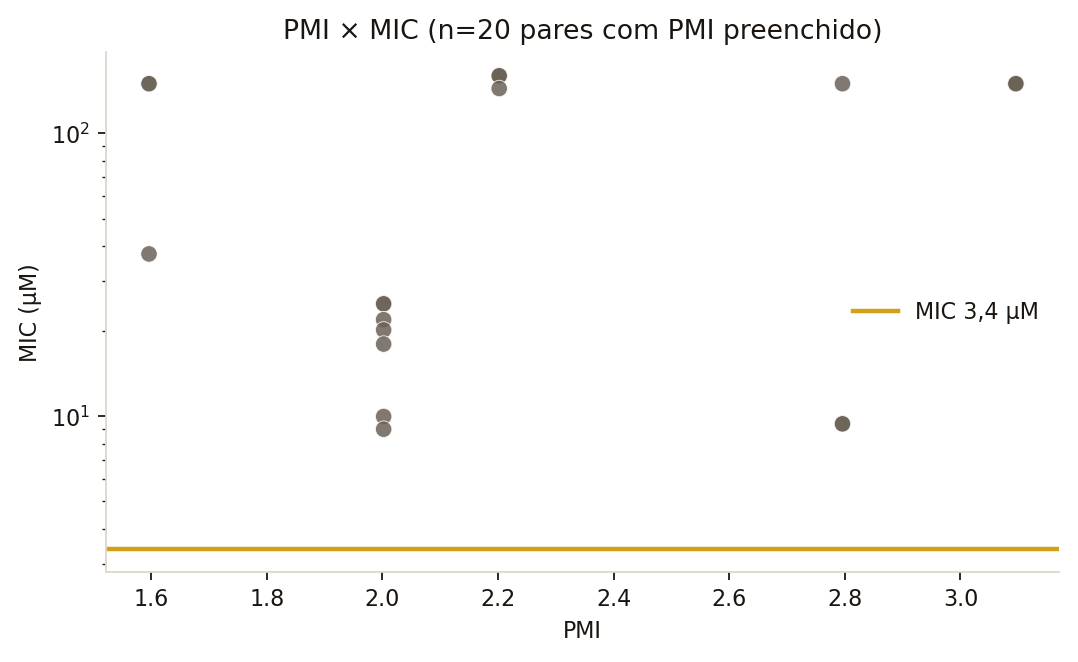
\includegraphics[width=0.95\linewidth]{pmi_vs_mic.png}
\end{center}
{\scriptsize PMI alto sugere interação favorável, mas \textbf{não garante} MIC baixo.}
}

\columnbreak

% ---------- COL 2 ----------
\sectionbox{4. Modelagem}{
\textbf{RF} (Nível 1 InovAI) · \texttt{Scaler}$\to$\texttt{RandomForest} · \texttt{class\_weight=balanced}\\
\textbf{LOPO} = métrica principal · LOO = referência · \textbf{isotônica} nas OOF LOPO

\vspace{0.15em}
\begin{center}
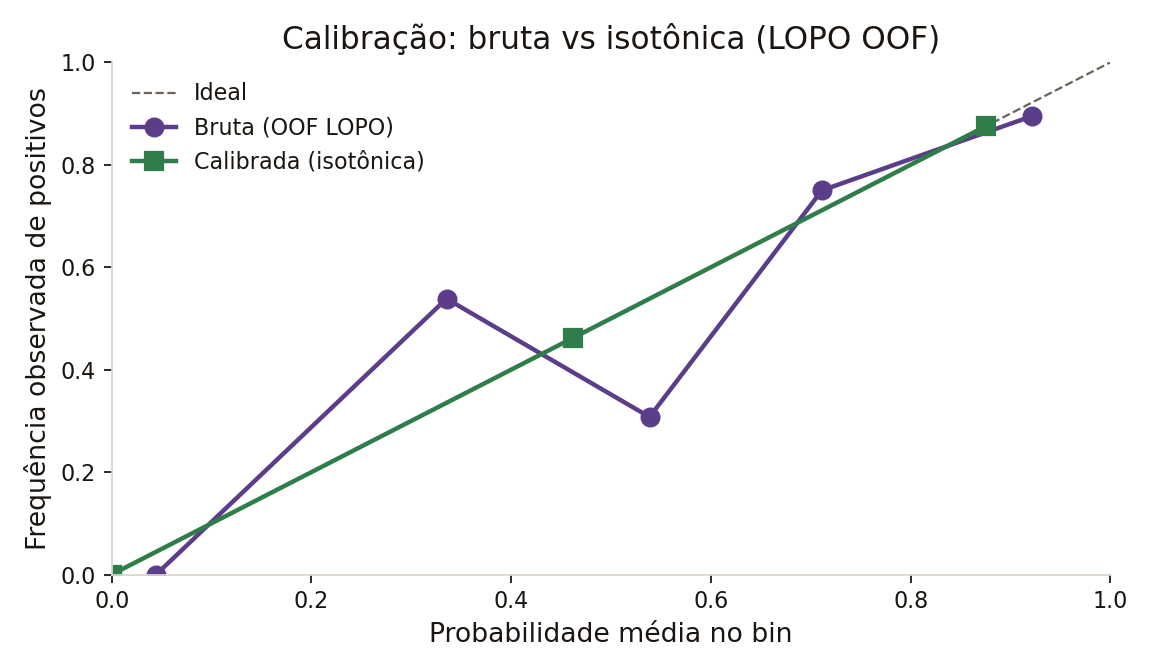
\includegraphics[width=0.95\linewidth]{calibracao.png}
\end{center}
}

\sectionbox{5. Resultados quantitativos}{
\begin{center}
\metriccard{Baseline RF}{0,85}{PmGreen}\hspace{0.2cm}%
\metriccard{Multimodal}{0,84}{PmVenomDeep}
\end{center}
\vspace{0.15em}
\begin{center}
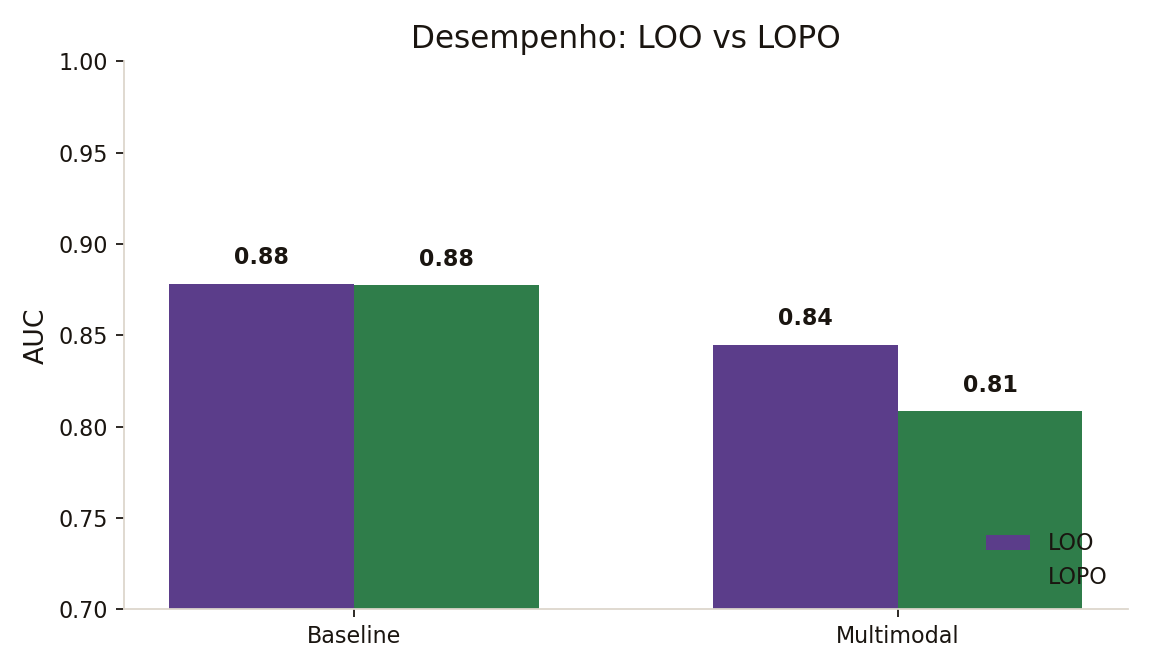
\includegraphics[width=0.95\linewidth]{auc_loo_lopo.png}\\[0.12em]
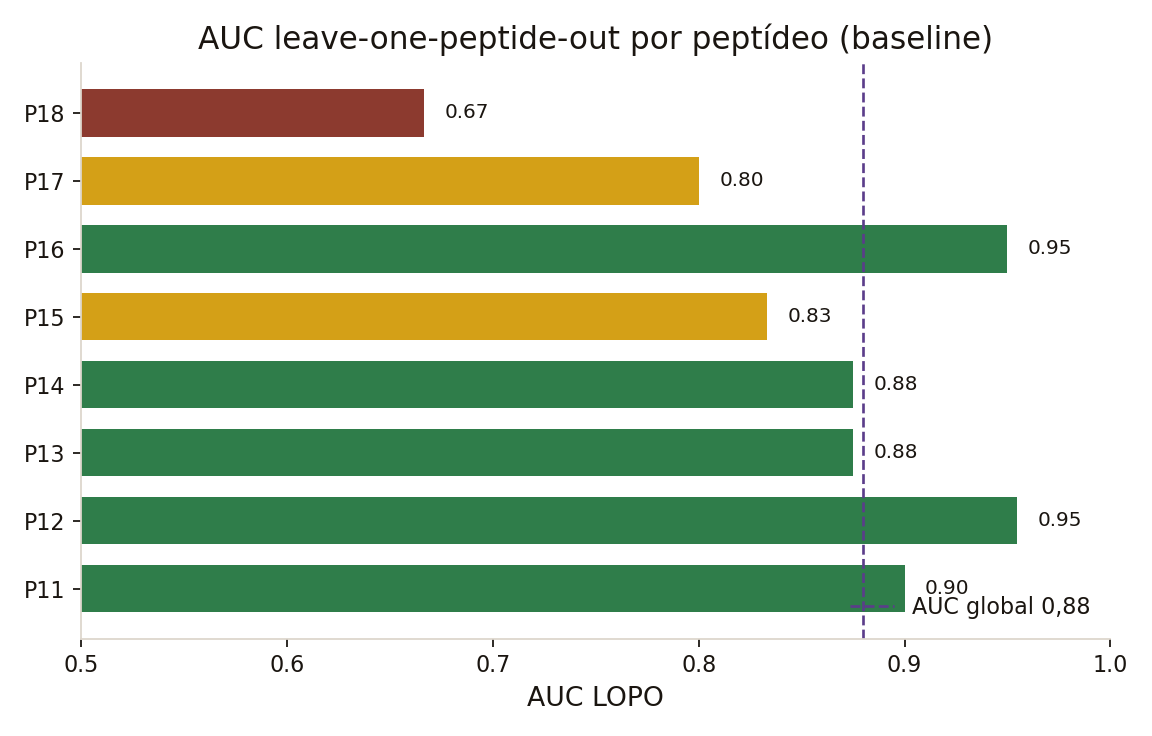
\includegraphics[width=0.95\linewidth]{auc_por_peptideo.png}\\[0.12em]
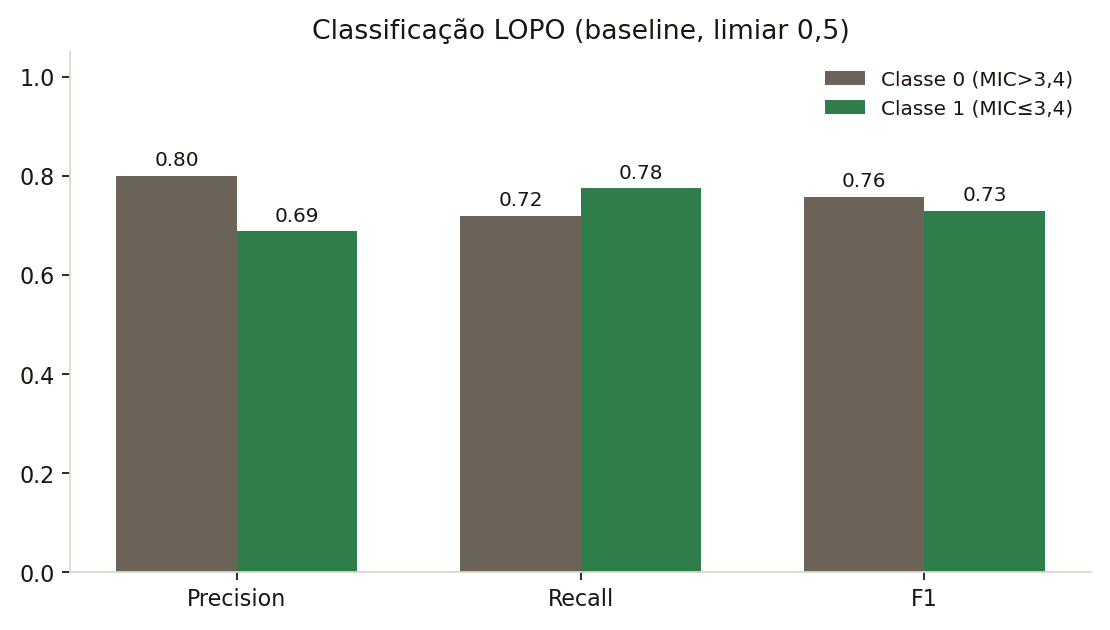
\includegraphics[width=0.95\linewidth]{classificacao_lopo.png}\\[0.12em]
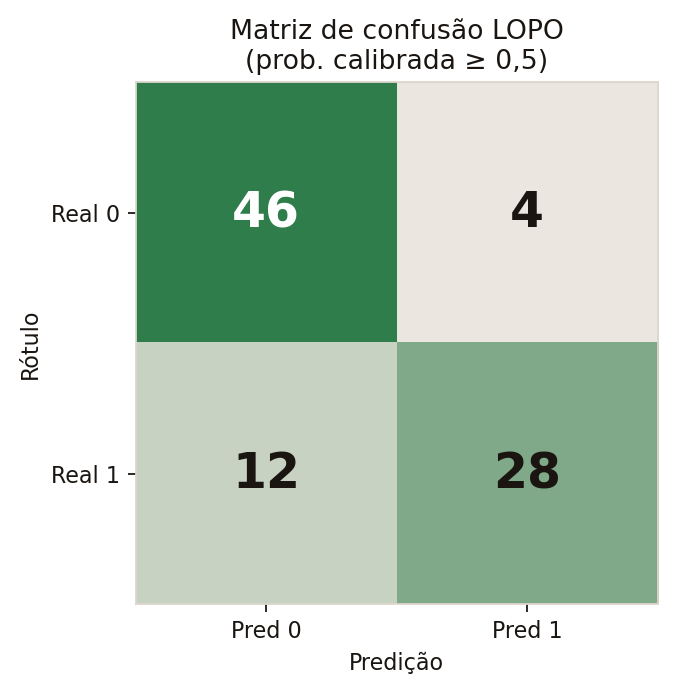
\includegraphics[width=0.62\linewidth]{matriz_confusao.png}
\end{center}
{\scriptsize Acc.\ LOPO baseline 0,77 · multimodal 0,80. Matriz: limiar 0,5 na prob.\ calibrada.}
}

\columnbreak

% ---------- COL 3 ----------
\sectionbox{6. Explicabilidade (SHAP)}{
TreeExplainer --- contribuição de cada descritor para alta atividade.

\vspace{0.12em}
\begin{center}
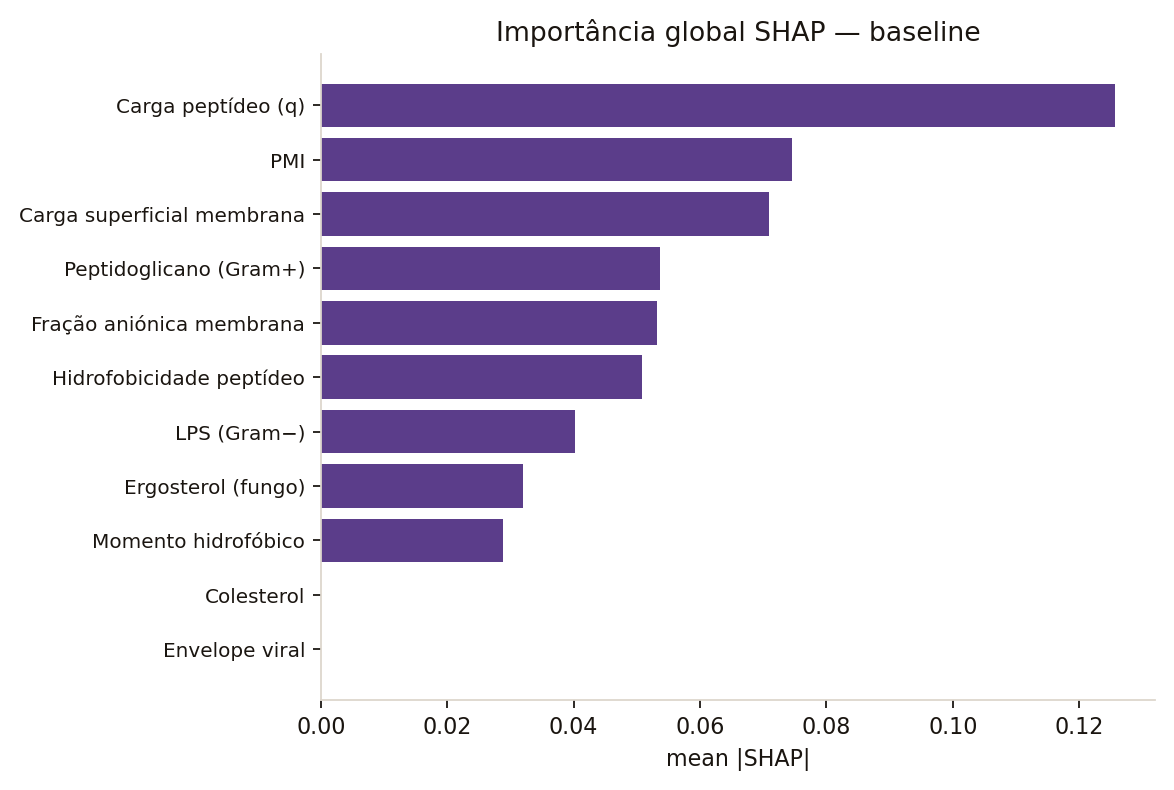
\includegraphics[width=0.95\linewidth]{shap_importancia.png}\\[0.12em]
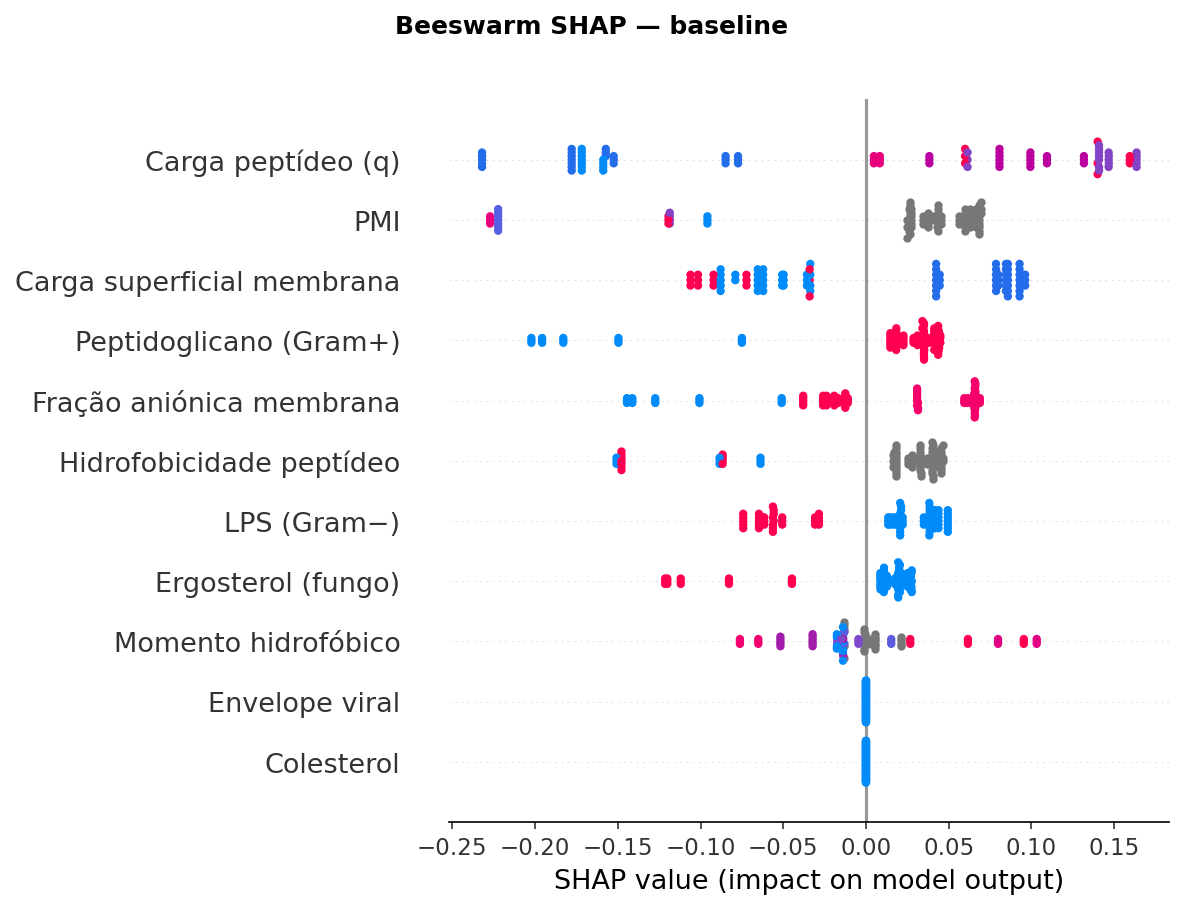
\includegraphics[width=0.95\linewidth]{shap_beeswarm_baseline.png}
\end{center}
{\scriptsize Top baseline: carga do peptídeo, PMI, carga superficial. ESM-2 agregado no multimodal.}
}

\sectionbox{7. Ranking e produto}{
Score multi-alvo: atividade $-$ $\lambda\cdot$toxicidade proxy ($cell\_normal$) + PMI\_sel.

\vspace{0.12em}
\begin{center}
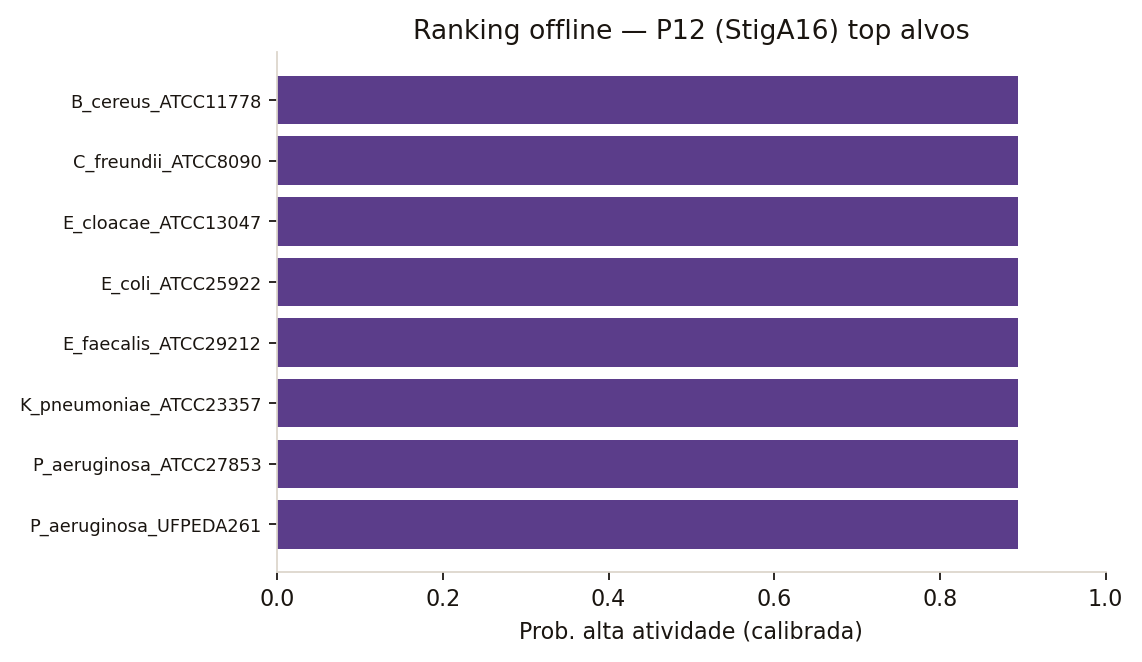
\includegraphics[width=0.95\linewidth]{ranking_p12.png}
\end{center}

\vspace{0.12em}
\begin{itemize}
  \item Dashboard: única / lote FASTA / ranking / relatórios MD·DOCX·PDF
  \item Cloud = baseline · Space HF = multimodal
  \item Faixas: $\ge$70\% priorizar · 40--70\% intermediário · $<$40\% baixa
\end{itemize}
}

\sectionbox{8. Limitações e conclusões}{
\textbf{Limitações:} $\sim$10 peptídeos; limiar operacional; RF não modela toxicidade direta; multimodal ainda não é DL completo.

\vspace{0.15em}
\textbf{Conclusões:}
\begin{enumerate}
  \item RF + PMI é robusto no PoC (Nível 1 InovAI)
  \item LOPO + isotônica tornam as \% interpretáveis
  \item Baseline LOPO AUC $\approx$\textbf{0,85}; multimodal $\approx$\textbf{0,84}
  \item Uso: \textbf{priorizar} análogos Stigmurin antes do in vitro
\end{enumerate}
\vspace{0.12em}
{\normalsize\texttt{github.com/gbmotta/PepMem-AI}}\\
{\scriptsize Parente 2022 · Lin et al.\ 2023 · Lee et al.\ 2016 · \texttt{docs/TREINO.md}}
}

\end{multicols}

\vspace{0.25cm}
\noindent
\begin{tikzpicture}
  \node[fill=PmPurple, minimum width=\linewidth, minimum height=2.0cm, inner sep=0] (f) {};
  \fill[PmPurpleSoft] ([yshift=1.82cm]f.south west) rectangle (f.north east);
  \node[anchor=west, fill=white, rounded corners=2pt, inner sep=5pt] at ([xshift=0.4cm]f.west)
    {
\includegraphics[height=1.0cm]{logos_inovai_ufrn.png}};
  \node[anchor=east, text=PmWhite, align=right] at ([xshift=-0.55cm]f.east) {%
    {\large\bfseries PepMem-AI \;$\cdot$\; PoC de priorização in vitro}\\[0.1em]
    {\normalsize InovAI Lab / UFRN --- 2026}%
  };
\end{tikzpicture}

\end{document}
